% THIS IS SIGPROC-SP.TEX - VERSION 3.1
% WORKS WITH V3.2SP OF ACM_PROC_ARTICLE-SP.CLS
% APRIL 2009
%
% It is an example file showing how to use the 'acm_proc_article-sp.cls' V3.2SP
% LaTeX2e document class file for Conference Proceedings submissions.
% ----------------------------------------------------------------------------------------------------------------
% This .tex file (and associated .cls V3.2SP) *DOES NOT* produce:
%       1) The Permission Statement
%       2) The Conference (location) Info information
%       3) The Copyright Line with ACM data
%       4) Page numbering
% ---------------------------------------------------------------------------------------------------------------
% It is an example which *does* use the .bib file (from which the .bbl file
% is produced).
% REMEMBER HOWEVER: After having produced the .bbl file,
% and prior to final submission,
% you need to 'insert'  your .bbl file into your source .tex file so as to provide
% ONE 'self-contained' source file.
%
% Questions regarding SIGS should be sent to
% Adrienne Griscti ---> griscti@acm.org
%
% Questions/suggestions regarding the guidelines, .tex and .cls files, etc. to
% Gerald Murray ---> murray@hq.acm.org
%
% For tracking purposes - this is V3.1SP - APRIL 2009

\documentclass{sig-alternate}
\usepackage{url}
\usepackage{etoolbox}
\usepackage{array}

\usepackage{caption}
\usepackage{wrapfig}

%this removes the copywright message as we dont need it
\patchcmd{\maketitle}{\@copyrightspace}{}{}{}

\begin{document}

\title{Byzantine Fault Tolerance in YARN}

%
% You need the command \numberofauthors to handle the 'placement
% and alignment' of the authors beneath the title.
%

\numberofauthors{4} %  in this sample file, there are a *total*
% of EIGHT authors. SIX appear on the 'first-page' (for formatting
% reasons) and the remaining two appear in the \additionalauthors section.
%
\author{
% You can go ahead and credit any number of authors here,
% e.g. one 'row of three' or two rows (consisting of one row of three
% and a second row of one, two or three).
%
% The command \alignauthor (no curly braces needed) should
% precede each author name, affiliation/snail-mail address and
% e-mail address. Additionally, tag each line of
% affiliation/address with \affaddr, and tag the
% e-mail address with \email.
%
% 1st. author
\alignauthor
Josh Fuerst\\
       \affaddr{Purdue University}\\
       \email{fuerst@purdue.edu}       
% 2nd. author
\alignauthor
Rachna Goyal\\
       \affaddr{Purdue University}\\
       \email{goyal15@purdue.edu}
\and 
% 3rd. author
\alignauthor 
Josh Reese\\
       \affaddr{Purdue University}\\
       \email{reese5@purdue.edu}
% 4th author
\alignauthor 
Derek Schatzlein\\
       \affaddr{Purdue University}\\
       \email{dschatzleinop@gmail.com}
}

\maketitle

\begin{abstract}
For this project we attempted to implement Byzantine Fault Tolerance (BFT) within YARN. The goal was to provide anyone using the 
YARN framework with the ability to have resources and tasks automatically duplicated. Our task focused specifically on the protion of 
BFT which deals with inconsistent output. 
\end{abstract}


\section{INTRODUCTION}

\begin{figure}
\centering
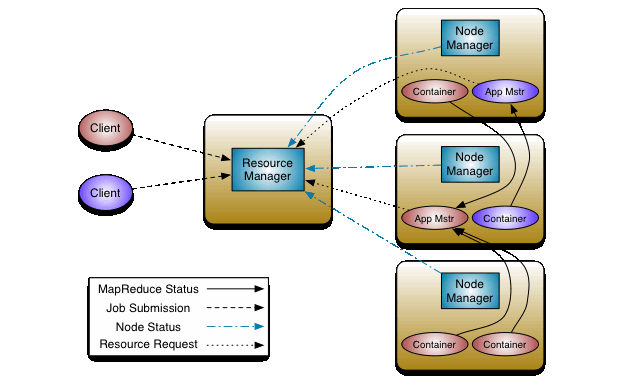
\includegraphics[width=10cm]{images/yarn_architecture.png}
\caption{YARN Architecture}
\label{fig:arch}
\end{figure}


Need to introduce some stuff here... bla bla bla fuck fuck fuck...
 
\section{RELATED WORK}
\label{sec:related}

Talk about Mesos, YARN, Spark, Byzantine Fault Tolerance





\begin{table*}
\centering
\begin{tabular}{|>{\bfseries}c|c|c|c|c|c|} \hline
\textbf{Method}    &    \textbf{Park Cost}    &    \textbf{User involvement}    &    \textbf{Accuracy}    &    \textbf{Automated}    &    \textbf{User Visibility}\\ \hline
Landmarks    &    None    &    Passive    &    Low    &    No    &    At Gate\\ \hline
Sensor Systems    &    High    &    Passive    &    High    &    Yes    &    At Gate/Online\\ \hline
Active Mobile Apps    &    None    &    Active    &    High/Low    &    Yes    &    Mobile Device (online)\\ \hline
Our Application    &    None    &    Passive    &    High/Low    &    Yes    &    Mobile Device (online)\\ \hline
\end{tabular}
\caption{Comparison of Queue Tracking Systems}
\label{tab:related_work}
\end{table*}
 
\section {SYSTEM DESIGN}
\label{sec:method}

Our system design began with just YARN in mind. Our hopes were to analyse the system and implement BFT entirely inside of YARN. Our hopes were to 
keep the YARN changes just within the API such that any future frameworks which use the same API's could utilize our changes. We also hoped that if 
our changes were within the standard API current YARN frameworks could have BFT without any changes. We later discovered that many current frameworks 
do not use YARN's API to handle the entire process. Spark is once such example. Spark uses the standard API to request containers.
 Spark however, starts its own separate scheduler which bypasses many of the communications needed to implement BFT. 


\subsection{YARN}
We used the provided examples within YARN to determine how the system functions. As it turns out YARN provides two simple classes AMRMClient and 
NMClient. AMRMClient handles the communication between the ApplicationMaster(AM) and the ResourceManager(RM). This is how the AM sends requests to the RM
for new containers. It is also how the RM reports back when the new containers are allocated. The NMClient class is what handles the communication between
the NodeManager(NM) and the AM. This is where the communication is sent to launch processes in the containers. 

Our system design creates a new class Byzantine. We altered the NMClient and AMRMClient classes to each create an instance of our Byzantine class. The overall idea
is that whenever there is a communication from AMRMClient or NMClient we intercept that communication. This means when the AM requests a container we can intercept that
resource request and replicated it. This means if we are in byantine mode, for each intercepted resource request we duplicate it so we have 4 total requests. As this is happening
we save off the request in a table. As the containers are allocated we intercept the communication from the RM back to the AM. We save each replica containers information
in the table with its respective resource request. This is done by matching the requested resources with those available in the container. 
We do not deliver the replica communication to the AM. Once all of the 
container replicas have been allocated we forward only one allocated container status back to the AM. We do this to hide all of the Byzantine replication from the AM. This means 
that existing AMs can run with our version of YARN with no changes. 

At this point the AM has received communication that one container has been allocated. This is the point where the AM will begin to form a ContainerLaunchContex. This encompasses the
information needed to run a task on the container. This includes a path to the .jar file which will be run on the container. Once the launch context is built the AM uses the NMClient
API to send communication to the launched container which tells it to start. At this point we intercept the communication and tell all of the containers replicas to perform the same
actions. We can do this because we have a table which maps each container to all of its replicas. 

At this point YARN will start running the provided task on the container. Upon completion the NM will report a completion status to the RM who forwards the status back to the AM via 
the AMRMClient API. In a similar fashion we intercept these communications. Again we hide the replicas completions from the AM. Once we have seen the completion status from all the 
replicas we must verify that they all have the same output. To do this we simply compare the output of each container. The containers output file name must be defined by a call 
to our Byzantine class. At this point if we have a successful Byzantine run we report that back to the AM. If not we report a Byzantine failure back to the AM. In the event of 
a Byzantine failure we assume it is up to the AM to decide what to do next. 



\subsection{Spark}
 

\section {EVALUATION}
\label{sec:evaluation}
Lorem ipsum dolor sit amet, consectetur adipiscing elit. Etiam id mauris adipiscing, pellentesque ligula sit amet, luctus leo. 
Duis congue nisl metus, id pretium nulla auctor vel. Lorem ipsum dolor sit amet, consectetur adipiscing elit. Sed mauris nisl, 
tincidunt nec purus sagittis, condimentum aliquet eros. Pellentesque eu dolor lectus. Nunc gravida, ipsum at pretium mollis, neque 
est porta massa, sed iaculis odio tellus vitae est. Nunc accumsan interdum condimentum. Fusce sit amet neque ut erat commodo molestie id ac est.

Nunc sagittis lacus mattis, lobortis nibh ac, varius justo. Aliquam vestibulum enim et molestie lobortis. Praesent magna nulla, auctor
egestas dictum quis, condimentum quis elit. Pellentesque iaculis bibendum pellentesque. Donec id semper sem. Nulla lacinia in leo fringilla 
laoreet. Integer in purus non nunc dapibus sagittis. Nunc dapibus neque nec ligula pretium, et rhoncus sapien pulvinar. Phasellus a enim rhoncus,
 ultricies tortor ut, vulputate enim. Aliquam odio orci, pharetra tempus ante at, mattis vehicula justo. Donec blandit ligula felis, placerat 
 fermentum nibh mollis sit amet. Nunc sed ultrices leo. Cras ut justo sed lacus accumsan condimentum sit amet in justo. Suspendisse dui diam, 
 venenatis a nisi at, sollicitudin gravida nisi.
 

\section{LIMITATIONS AND FUTURE WORK}
\label{sec:future}
Lorem ipsum dolor sit amet, consectetur adipiscing elit. Etiam id mauris adipiscing, pellentesque ligula sit amet, luctus leo. 
Duis congue nisl metus, id pretium nulla auctor vel. Lorem ipsum dolor sit amet, consectetur adipiscing elit. Sed mauris nisl, 
tincidunt nec purus sagittis, condimentum aliquet eros. Pellentesque eu dolor lectus. Nunc gravida, ipsum at pretium mollis, neque 
est porta massa, sed iaculis odio tellus vitae est. Nunc accumsan interdum condimentum. Fusce sit amet neque ut erat commodo molestie id ac est.

Nunc sagittis lacus mattis, lobortis nibh ac, varius justo. Aliquam vestibulum enim et molestie lobortis. Praesent magna nulla, auctor
egestas dictum quis, condimentum quis elit. Pellentesque iaculis bibendum pellentesque. Donec id semper sem. Nulla lacinia in leo fringilla 
laoreet. Integer in purus non nunc dapibus sagittis. Nunc dapibus neque nec ligula pretium, et rhoncus sapien pulvinar. Phasellus a enim rhoncus,
 ultricies tortor ut, vulputate enim. Aliquam odio orci, pharetra tempus ante at, mattis vehicula justo. Donec blandit ligula felis, placerat 
 fermentum nibh mollis sit amet. Nunc sed ultrices leo. Cras ut justo sed lacus accumsan condimentum sit amet in justo. Suspendisse dui diam, 
 venenatis a nisi at, sollicitudin gravida nisi.
 
\section{CONCLUSIONS}
\label{sec:conclusions}
Lorem ipsum dolor sit amet, consectetur adipiscing elit. Etiam id mauris adipiscing, pellentesque ligula sit amet, luctus leo. 
Duis congue nisl metus, id pretium nulla auctor vel. Lorem ipsum dolor sit amet, consectetur adipiscing elit. Sed mauris nisl, 
tincidunt nec purus sagittis, condimentum aliquet eros. Pellentesque eu dolor lectus. Nunc gravida, ipsum at pretium mollis, neque 
est porta massa, sed iaculis odio tellus vitae est. Nunc accumsan interdum condimentum. Fusce sit amet neque ut erat commodo molestie id ac est.

Nunc sagittis lacus mattis, lobortis nibh ac, varius justo. Aliquam vestibulum enim et molestie lobortis. Praesent magna nulla, auctor
egestas dictum quis, condimentum quis elit. Pellentesque iaculis bibendum pellentesque. Donec id semper sem. Nulla lacinia in leo fringilla 
laoreet. Integer in purus non nunc dapibus sagittis. Nunc dapibus neque nec ligula pretium, et rhoncus sapien pulvinar. Phasellus a enim rhoncus,
 ultricies tortor ut, vulputate enim. Aliquam odio orci, pharetra tempus ante at, mattis vehicula justo. Donec blandit ligula felis, placerat 
 fermentum nibh mollis sit amet. Nunc sed ultrices leo. Cras ut justo sed lacus accumsan condimentum sit amet in justo. Suspendisse dui diam, 
 venenatis a nisi at, sollicitudin gravida nisi.
 

% The following two commands are all you need in the
% initial runs of your .tex file to
% produce the bibliography for the citations in your paper.
\bibliographystyle{abbrv}
\bibliography{references}  % references.bib is the name of the Bibliography in this case

\balancecolumns
\end{document}